%% LyX 1.3 created this file.  For more info, see http://www.lyx.org/.
%% Do not edit unless you really know what you are doing.
\documentclass[english, 12pt]{article}
\usepackage{times}
%\usepackage{algorithm2e}
\usepackage{url}
\usepackage{bbm}
\usepackage[T1]{fontenc}
\usepackage[latin1]{inputenc}
\usepackage{geometry}
\geometry{verbose,letterpaper,tmargin=2.5cm,bmargin=2.5cm,lmargin=2.5cm,rmargin=2.5cm}
\usepackage{rotating}
\usepackage{color}
\usepackage{graphicx}
\usepackage{amsmath, amsthm, amssymb}
\usepackage{setspace}
\usepackage{lineno}
\usepackage{hyperref}
\usepackage{bbm}


\linenumbers
\doublespacing
%\usepackage[authoryear]{natbib}
\usepackage{natbib} \bibpunct{(}{)}{;}{author-year}{}{,} 

%Pour les rajouts
\usepackage{color}
\definecolor{trustcolor}{rgb}{0,0,1}

\usepackage{dsfont}
\usepackage[warn]{textcomp}
\usepackage{adjustbox}
\usepackage{multirow}
\usepackage{graphicx}
\graphicspath{{../figures/}}
\DeclareMathOperator*{\argmin}{\arg\!\min}

\let\tabbeg\tabular
\let\tabend\endtabular
\renewenvironment{tabular}{\begin{adjustbox}{max width=\textwidth}\tabbeg}{\tabend\end{adjustbox}}

\makeatletter

%%%%%%%%%%%%%%%%%%%%%%%%%%%%%% LyX specific LaTeX commands.
%% Bold symbol macro for standard LaTeX users
%\newcommand{\boldsymbol}[1]{\mbox{\boldmath $#1$}}

%% Because html converters don't know tabularnewline
\providecommand{\tabularnewline}{\\}

\usepackage{babel}
\makeatother


\begin{document}


\title{Predicting complex diseases: performance, robustness and ..utility..(impact?)}
\author{Florian Priv\'e\,$^{\text{ 1,}*}$, Hugues Aschard\,$^{\text{2,3}}$ and Michael G.B. Blum\,$^{\text{1,}*}$}



\date{~ }
\maketitle

\noindent$^{\text{\sf 1}}$Universit\'e Grenoble Alpes, CNRS, Laboratoire TIMC-IMAG, UMR 5525, France, \\
\noindent$^{\text{\sf 2}}$Centre de Bioinformatique, Biostatistique et Biologie Int\'egrative (C3BI), Institut Pasteur, Paris, France \\
\noindent$^{\text{\sf 3}}$Department of Epidemiology, Harvard T.H. Chan School of Public Health, Boston, Massachusetts, USA.

\noindent$^\ast$To whom correspondence should be addressed.

\newpage
\abstract{
\textbf{Motivation:} \\
\textbf{Results:} \\
\textbf{Availability:} \\
\textbf{Contact:} \href{florian.prive@univ-grenoble-alpes.fr}{florian.prive@univ-grenoble-alpes.fr} \& \href{michael.blum@univ-grenoble-alpes.fr}{michael.blum@univ-grenoble-alpes.fr}\\
\textbf{Supplementary information:}
}

%%%%%%%%%%%%%%%%%%%%%%%%%%%%%%%%%%%%%%%%%%%%%%%%%%%%%%%%%%%%%%%%%%%%%%%%%%%%%%%%

\newpage
\section{Introduction}

Polygenic Risk Scores (PRSs) combine the information contained in many single-nucleotide polymorphisms (SNPs) in a score that aims at reflecting the risk of developing a disease for which this score has been created. PRSs have proven to be useful for different applications, such as finding a common genetic contribution between two diseases \cite[]{purcell2009common}. 
Personalized medicine is another major application of PRSs. Personalized medicine will use PRSs in screening campaigns in order to identify high-risk individuals for a given disease. As an example of practical application, targeting screening to men at higher polygenic risk could reduce the problem of overdiagnosis and lead to a better benefit-to-harm balance in screening for prostate cancer \cite[]{pashayan2015implications}. Moreover, screening based on sequencing seems to make individuals positively change their health behavior while not causing patient anxiety nor depression \cite[]{vassy2017impact}.
Yet, PRSs would have to show a high discriminative power between cases and controls in order to be used for helping in the diagnosis of diseases. For example, for respectively screening high-risk individuals and for presymptomatic diagnosis of the general population, it is suggested that the AUC must be greater than respectively 75\% and 99\% \cite[]{janssens2007impact}.

Many methods have been developed in order to maximize the predictive power of genotypes for diseases, or more generally for phenotypes.
A commonly used technique, called P+T (which stands for ``Pruning and Thresholding'') -- or genetic profiling ..or even just PRS.. -- is used to derive PRSs from results of Genome-Wide Association Studies (GWASs) \cite[]{chatterjee2013projecting,dudbridge2013power,evans2009harnessing,purcell2009common,wray2007prediction}. This technique only use summary statistics which makes it very ..suitable.. and also very fast.
Linear Mixed-Models (LMMs) are another widely-used method in fields such as plant and animal breeding or for predicting highly heritable quantitative human phenotypes such as height \cite[]{lello2017accurate,yang2010common}. Yet, these models are not ..constructed.. for predicting a binary trait such as a disease status and have proven to ..fail.. at such task in another comparative study \cite[]{abraham2013performance}. Moreover, these methods and their ..derivations.. are often computationally demanding, both in terms of memory and time ..requirements.., which makes them unlikely to be used for prediction on large cohorts \cite[]{golan2014effective,maier2015joint,speed2014multiblup,zhou2013polygenic}.
Statistical learning methods have also been used to derive PRSs for complex human disease by jointly estimating SNP effects. Such methods include logistic regression, Support Vector Machine (SVM) and random forests \cite[]{abraham2012sparsnp,abraham2014accurate,botta2013walk,botta2014exploiting,wei2009disease}.

We recently developed two R packages, bigstatsr and bigsnpr, for efficient management and analysis of large-scale genome-wide data \cite[]{prive2017efficient}. Package bigstatsr includes efficient functions for computing penalized linear and logistic regressions on huge datasets. In this paper, we present a comprehensive comparative study of the P+T method, our penalized logistic regression and finally the T-Trees algorithm, which is a derivation of random forests and has shown exceptionally good predictive results in \cite{botta2014exploiting}. 
Note that the SVM model is expected to give similar results to logistic regression \cite[]{abraham2012sparsnp} and therefore isn't added to the comparison.
For the P+T model, we compare different thresholds of inclusion of SNPs.
For the logistic regression, we include two novel approaches. 
First, we introduce a procedure that we call Cross-Model Selection and Averaging (CMSA) for choosing the amount of regularization used, which directly affects the number of SNPs included in the model. 
We also show how to use feature engineering in order to capture not only linear effects, but also recessive and dominant effects.

There have already been comparative studies about predicting human binary phenotypes based on genotype data. 
\citep{abraham2013performance} showed that penalized logistic regression and penalized SVM performed better than the standard P+T method and LMMs, for a wide-range of human diseases.
\cite{zhou2013polygenic} used simulations on real genotypes of Australian individuals to show that a hybrid of linear mixed models and sparse regression models performed better in a range of sparse to polygenic disease architectures. 
\cite{spiliopoulou2015genomic} investigated the effect of relatedness in prediction performance.
\cite{ware2017heterogeneity} evaluated best practices for using the P+T method and found out, for example, that the optimal inclusion threshold is trait-dependent. 
In this study, we particularly extend the work of \cite{abraham2013performance} by using a simulation framework similar but ..richer.. than the one used in \cite{zhou2013polygenic}. In order to make our comparison as comprehensive as possible, we compare different architectures of disease (number, size and location of causal effects and heritability) with different model of generating liability ..scores.., one with only linear effects, and one which combines linear, dominant and interaction effects. First, we quickly discard T-Trees as being the best method for predicting disease status based on genotypes.
Then, we show that penalized logistic regression consistently performs better than the P+T method whereas predictive performance of the P+T method is very sensitive to the threshold of inclusion of SNPs, depending of the architecture of disease, as shown in \cite{ware2017heterogeneity}.


%%%%%%%%%%%%%%%%%%%%%%%%%%%%%%%%%%%%%%%%%%%%%%%%%%%%%%%%%%%%%%%%%%%%%%%%%%%%%%%%

\section{Methods}

\subsection{Genotype data}

We use real genotypes of European individuals from a case/control celiac disease cohort \cite[]{dubois2010multiple}. Composition of this dataset is presented in table \ref{tab:celiac-data}.
Details of quality control and imputation for this dataset are available in \cite{prive2017efficient}.
For simulations, in order to remove the structure induced by the celiac disease status, we first keep only controls from this cohort. Secondly, in order to remove population structure, we keep only people from the UK. Thirdly, we further subset these British people based on deviation of robust Mahalanobis distance on principal components. This 3-step filtering results in 7102 individuals with minimal population structure (see ..SupMat..). We decided to get rid of population structure because it can affect the predictive performance of methods, which we will investigate in another study.


\subsection{Simulations of phenotypes} \label{sec:simus}

To simulate phenotypes, we use the Liability Threshold Model (LTM) with a prevalence of 30\%. We vary different parameters: the number of chromosomes used (either all 22 chromosomes or only the chromosome 6), the size of the training set (from 1000 to 6000 by 1000, and the corresponding test set is composed of the remaining individuals), the number of causal variants and their location (30, 300 or 3000 anywhere on the dataset or 30 only in the HLA region), the heritability (50\% or 80\%), the distribution of effects associated with causal SNPs (Normal or Laplace), and the model used to generate the genetic ..part.. of the phenotypes (one ``simple model'' with only linear effects, and one ``fancy model'' which combines linear, dominant and interaction effects).
For the ``simple model'', we compute $$y_i = \sum_{j\in E_\text{causal}} w_j \cdot \widetilde{G_{i,j}}$$ where $w_j$ are weights (generated with a Gaussian or a Laplace distribution), $G_{i,j}$ is the allele count of individual $i$ for SNP $j$ and $\widetilde{G_{i,j}}$ corresponds to its standardized version (zero mean and unit variance for all SNPs). 
For the ``fancy model'', we separate the causal SNPs in three equal sets $E_\text{causal}^{(1)}$, $E_\text{causal}^{(2)}$ 
and $E_\text{causal}^{(3)}$ ($E_\text{causal}^{(3)}$ is further separated in two equal sets, $E_\text{causal}^{(3.1)}$ and $E_\text{causal}^{(3.2)}$). We then compute $$y_i = \underbrace{\sum_{j\in E_\text{causal}^{(1)}} w_j \cdot \widetilde{G_{i,j}}}_\text{linear} + \underbrace{\sum_{j\in E_\text{causal}^{(2)}} w_j \cdot \widetilde{D_{i,j}}}_\text{dominant} + \underbrace{\sum_{\substack{k=1 \\ j_1=e_k^{(3.1)} \\ j_2=e_k^{(3.2)}}}^{k=\left|E_\text{causal}^{(3.1)}\right|} w_{j_1} \cdot \widetilde{G_{i,j_1} G_{i,j_2}}}_\text{interaction}$$ where $D_{i,j} = \mathds{1}\left\{G_{i,j} \neq 0\right\}$ and $E_\text{causal}^{(q)}=\left\{e_k^{(q)},~k \in \left\{1, \ldots, \left|E_\text{causal}^{(q)}\right|\right\}\right\}$. Note that for the interaction part of the model, we scale interactions, not the raw allele counts, so that corresponding SNPs still display a marginal effect. 
For both models, the $y_i$ are then standardized such that they have a variance equal to the desired heritability $h^2$ and we further add some environmental noise $\epsilon_i$ to $y_i$ where $\epsilon \sim N(0, 1 - h^2)$.

We make 5 different simulation procedures, summarized in table \ref{tab:simus}. 
..Simulation.. \textnumero1 uses the whole dataset (the 22 chromosomes), a training set of size 6000 and an heritability of 80\%. It compares all methods (see section \ref{sec:methods}) on all other combination of parameters in 5 simulations. The goal of the first simulation is to quickly discard the T-Trees method.
For simulation \textnumero2, we make also vary the heritability (50\% or 80\%) but we don't run the T-Trees method anymore. The goal of the second simulation is to compare all remaining methods, especially to see how well the ``logit-triple'' method works. We run 20 simulations for each combination of parameters.
For simulation \textnumero3, we continue with 80 more simulations (to reach 100 simulations, i.e.\ 5 times more than in \cite{zhou2013polygenic}), but discarding the ``logit-triple'' method and the ``fancy'' model. 
Simulation \textnumero4 consists in 100 simulations of remaining methods and combinations of parameters on a dataset composed of only the chromosome 6. Reducing the number of SNPs aims at increasing the ..polygenicity.. of our simulated models and at ..virtually.. increasing the sample size [REF? DUDBRIDGE?]. 
Finally, simulation \textnumero5 reuses the whole dataset but varying the size of the training set in order to assess how the number of samples affects predictive performance of the PRS and the ``logit-simple'' methods. 100 simulations are run using 300 causal SNPs anywhere on the genome. 


\subsection{Predictive performance measures}

In this study, we use two different measures of predictive accuracy. 
First, we use the Area Under the Receiver Operating Characteristic (ROC) Curve (AUC) \cite[]{fawcett2006introduction,hanley1982meaning,lusted1971signal}. In the case of our study, the AUC is the probability that a PRS of a case is greater than the PRS of a control.
This measure indicates how well we can distinguish between cases and controls using PRSs.
As a second measure, we report the percentage of cases in the 10\% and 20\% largest PRSs. This measure indicates how well we can identify high-risk individuals from a higher PRS in screening campaigns.
[COMMENT ON PREVALENCE?]

Note that we also report the timing of the main computations and the number of SNPs used in the predictions.

\subsection{Compared methods} \label{sec:methods}

In this study, we compare three different types of methods: the P+T method, the T-Trees method and a penalized logistic regression.

The P+T (Pruning + Thresholding) method directly derives a Polygenic Risk Score (PRS) from the results of Genome-Wide Associations Studies (GWASs), called summary statistics.
For the P+T method, a coefficient of regression is learned independently for each SNP along with a corresponding p-value (the GWAS part). 
The SNPs are first clumped (P) so that there remain only loci that are weakly correlated with each other. 
Then, thresholding (T) consists in removing SNPs that are within a certain level of significance (p-value threshold to be determined). 
Finally, a polygenic risk score is defined as the sum of allele counts of the remaining SNPs weighted by the corresponding effect coefficients: $$S_i(T) = \sum_{j \in E_\text{clumping}} \mathds{1}\{p_j < T\} \cdot \beta_j \cdot G_{i,j}$$ where $\beta_j$ ($p_j$) are the effect sizes (p-values) learned from the GWAS and $T$ is a threshold on p-values to be determined. In this study, we report scores for a clumping threshold at $r^2 > 0.2$ within regions of 500kb. 

For the P+T method, we report three different scores of prediction: one including all the SNPs (remaining after clumping), one including only SNPs that have a p-value under the GWAS threshold of significance ($p < 5 \cdot 10^{-8}$), and one that maximizes the AUC for these two thresholds and a sequence of 100 values of thresholds ranging from $10^{-0.1}$ to $10^{-100}$ and equally spaced on the log-log-scale (Table \ref{tab:thr}). Note that, normally, the optimal threshold would have to be learned on the training set only. We consider this reported maximum AUC as an upper bound of the AUC for the P+T method.
We call these three reported scores respectively ``PRS-all'', ``PRS-stringent'' and ``PRS-max'' in the results.

T-Trees (\textit{Trees inside Trees}) is an algorithm derived from random forests \cite[]{breiman2001random} that takes into account the correlation structure among the genetic markers implied by linkage disequilibrium in GWAS data \cite[]{botta2014exploiting}. Since this method is significantly different from the other tested here and achieved surprisingly results in the past, we decided to include T-Trees in this comparison in order to assess whether or not it could give superior predictive performance. We use the same parameters as reported in Table 4 of \cite{botta2014exploiting}. Yet, we use only 100 trees (instead of 1000) because it showed only a very subtle increase of AUC while taking way too much time (e.g.\ AUC of 81.5\% instead of 81\%, data not shown). %We call this method ``T-Trees'' in the results.


The last method we compare is penalized logistic regression.
We solve: $$\argmin_{\beta_0, \beta}(x, y, \lambda)\left\{\underbrace{\frac{1}{n}\sum_{i=1}^n \log\left(1+e^{-y_i (\beta_0+x_i^T\beta)}\right)}_\text{Loss function} + \underbrace{\lambda \left((1-\alpha)\frac{1}{2}\|\beta\|_2^2 + \alpha \|\beta\|_1\right)}_\text{Penalization}\right\}$$ where, in this study, $x$ is the genotypes and covariables (e.g.\ principal components), $y$ is the disease status we want to predict and $\lambda$ is a regularization parameter that need to be determined. 
Different regularizations can be used to prevent overfitting, among other benefits: the L2-regularization (ridge, \cite{hoerl1970ridge}) shrinks coefficients and is ideal if there are many predictors drawn from a Gaussian distribution (corresponds to $\alpha = 0$ in the previous equation),
 the L1-regularization (lasso, \cite{tibshirani1996regression}) forces some of the coefficients to be exactly zero and can be used as a means of variable selection, leading to sparse (and therefore more interpretable) models  (corresponds to $\alpha = 1$), 
the L1- and L2-regularization (elastic-net, \cite{zou2005regularization}) is a compromise between the two previous penalties and is particularly useful in the $m \gg n$ situation ($m$: number of SNPs), or any situation where there are many correlated predictors (corresponds to $0 < \alpha < 1$) \cite[]{friedman2010regularization}. In this study, we always use the elastic-net regularization with $\alpha = 0.5$, without trying to tune (e.g.\ by grid-search and cross-validation) the value of this hyper-parameter $\alpha$.

To fit this penalized logistic regression, we use a very efficient algorithm \cite[]{friedman2010regularization,tibshirani2012strong,zeng2017efficient}, also implemented in our package bigstatsr \cite[]{prive2017efficient}. 
This type of algorithm builds predictions for many values of $\lambda$ (typically a ``regularization path'' of 100 values). To get an algorithm free of the choice of this hyper-parameter $\lambda$, we developed a procedure that we called Cross-Model Selection and Averaging (CMSA). First, this procedure separates the training set in $K$ folds (e.g.\ 10 folds). Secondly, in turn, each fold is considered as an inner validation set and the others ($K - 1$) folds form an inner training set, the model is trained on the inner training set and the corresponding predictions (scores) for the inner validation set are computed, the vector of scores which maximizes a criterion (e.g.\ AUC) is determined and the vector of coefficients corresponding to the previous vector of scores is chosen. Finally, the $K$ resulting vectors of coefficients are combined into one vector (e.g.\ using the geometric median). Because of L1-regularization, this vector of coefficients is typically very sparse and can be used to make a PRS based on a \textit{linear} combination of allele counts. We call this method ``logit-simple'' in the results.

In order to capture recessive and dominant effects in addition to linear effects, we use feature engineering: we construct another dataset with, for each SNP variable, two more variables coding for recessive and dominant effects. This results in a dataset with 3 times more variables than the initial one, on which we can apply the standard logistic regression with the CMSA procedure, described previously. We call this method ``logit-triple'' in the results.

\subsection{Reproduciblity}

All the code used in this paper along with results such as figures and tables, are available as HTML R notebooks in the Supplementary Materials.

%%%%%%%%%%%%%%%%%%%%%%%%%%%%%%%%%%%%%%%%%%%%%%%%%%%%%%%%%%%%%%%%%%%%%%%%%%%%%%%%

\section{Results}

[MONTRER UN MANHATTAN PLOT POUR JUSTIFIER 30 IN HLA]

[MONTRER UN GRAPH EN FCT D'INCLUSION]

\subsection{Overview and naming}

\subsection{T-Trees}

First, we ran only 5 simulations for each combination of parameters), excepted for the heritability that we fixed at $0.8$ (see section \ref{sec:simus}).
The goal was to quickly discard the T-Trees method as being competitive with the other methods. 
For example, compared to our penalized logistic regression, T-Trees perform worse for both predictive measures, the AUC and the percentage of cases in highest scores (Figure \ref{fig:ttrees}). Moreover, T-Trees takes longer to run and makes more complex predictive models because it uses more SNPs in the models and has non-linear effects (Figure \ref{fig:ttrees}).
So, we decided to discard this method for the rest of the simulations.

\subsection{Main simulations}

[Also return p-values?]\\

First, we show that AUC is highly correlated ($r^2 > 95\%$) with the percentage of cases in either the 10\% or 20\% largest PRSs (Figure \ref{fig:AUC-corr}). Therefore, AUC can be a good measure at determining whether a score can identify high-risk individuals or not, so we report only predictive performance in terms of AUC in the following results.

Using the penalized logistic regressions, we report AUCs greater than 95\%, which is not obtained by the upper bound of the P+T method in any scenario (Figure \ref{fig:AUC}). Our penalized regression methods consistently provides better predictive performance than the P+T method for all disease architectures tested [ou pas, FIGURE]. Our method is parallelized and requires only less than 10 minutes to run (with 6 physical cores) [TABLE ?FIGURE?]. Moreover, it results in relatively sparse models with no more than 14,000 predictors entering the models even for the linear model of 3000 causal SNPs [TABLE ?FIGURE?].
P+T runs in only a few seconds because we don't consider the GWAS computation as part of the execution time of the method because this is generally executed by others (e.g.\ consortia) and then only the resulting summary statistics are used to construct a PRS. 

As for the comparison between our two penalized logistic regression, the classic one (called ``simple'') and the one using additional features coding for recessive and dominant effects (called ``triple''), we report that the ``triple'' method is nearly as good as the ``simple'' one when there are only linear effects and can lead to significantly greater results when there are also dominant and interactions effects (Figure \ref{fig:AUC-rel}). Yet, the ``triple'' solution takes approximately 3 more times to run.

As for general results, we report a decrease of AUC when the number of causal variants $M$ is increasing [BATEAU? quoi d'autre?].

[TROUVER DES AUTRES: \% of decrease for h2 0.8 -> 0.5? Pas bon d'utliser tous les SNPs]

\subsection{Simulations varying training size and number of SNPs}

\section{Discussion}

In this comparative study, we proposed other methods as a replacement to the widely used P+T method. 
We show that jointly estimating the SNP effects using efficient penalized logistic regressions enable to achieve really good performance, as reported in a previous study \cite[]{abraham2013performance}, higher than with the P+T method.
We are well aware that the P+T method is widely used because it is simple and can use summary statistics already learned from large genotype data, which is not the case for our penalized logistic regressions. 
Yet, in the case of prediction of disease to be used for clinical interventions, best possible methods should be used, even if it has to be used by large consortia only [EVEN LARGE CONSORTIA DON'T HAVE ALL DATA?].

One does not simply identify high-risk individuals (Figure \ref{fig:meme}).


[PARLER DU PROBLEME DE POP? + future paper]


\newpage
\begin{table}[htbp]
\caption{Summary of all simulations. When there is symbol `-' in a box, it means that the parameters are the same as the ones in the upper box.}
\vspace*{0.5em}
\begin{tabular}{|c|c|c|c|c|c|c|c|c|}
\hline
Numero of & \multirow{2}{*}{Dataset} & Size of & Causal SNPs & Distribution & \multirow{2}{*}{Heritability} & Simulation & Number of & \multirow{2}{*}{Methods} \\ 
simulation & & training set & (number and location) & of effects & & model & simulations & \\
\hline
\hline
\multirow{4}{*}{1} & \multirow{4}{*}{All 22 chromosomes} & \multirow{4}{*}{6000} & 30 in HLA & \multirow{2.5}{*}{Gaussian} & \multirow{4}{*}{0.8} & \multirow{2.5}{*}{simple} & \multirow{4}{*}{5} & PRS \\
& & & 30 in all & & & & & logit-simple \\
& & & 300 in all & \multirow{1.5}{*}{Laplace} & & \multirow{1.5}{*}{fancy} & & logit-triple \\
& & & 3000 in all & & & & & T-Trees \\
\hline
\multirow{3}{*}{2} & \multirow{3}{*}{-} & \multirow{3}{*}{-} & \multirow{3}{*}{-} & \multirow{3}{*}{-} & \multirow{2}{*}{0.5} & \multirow{3}{*}{-} & \multirow{3}{*}{20} & PRS \\ 
& & & & & \multirow{2.2}{*}{0.8} & & & logit-simple \\
& & & & & & & & logit-triple \\
\hline
\multirow{2}{*}{3} & \multirow{2}{*}{-} & \multirow{2}{*}{-} & \multirow{2}{*}{-} & \multirow{2}{*}{-} & \multirow{2}{*}{-} & \multirow{2}{*}{simple} & \multirow{2}{*}{80} & PRS \\ 
& & & & & & & & logit-simple \\
\hline
\multirow{2}{*}{4} & \multirow{2}{*}{Chromosome 6 only} & \multirow{2}{*}{-} & \multirow{2}{*}{-} & \multirow{2}{*}{-} & \multirow{2}{*}{-} & \multirow{2}{*}{-} & \multirow{2}{*}{100} & \multirow{2}{*}{-} \\ 
& & & & & & & & \\
\hline
\multirow{5}{*}{5} & \multirow{5}{*}{All 22 chromosomes} & 1000 & \multirow{5}{*}{300 in all} & \multirow{5}{*}{-} & \multirow{5}{*}{-} & \multirow{5}{*}{-} & \multirow{5}{*}{100} & \multirow{5}{*}{-} \\ 
& & 2000 & & & & & & \\
& & 3000 & & & & & & \\
& & 4000 & & & & & & \\
& & 5000 & & & & & & \\
\hline
\end{tabular}
\label{tab:simus}
\end{table}


\newpage
\begin{figure}[h]
\centerline{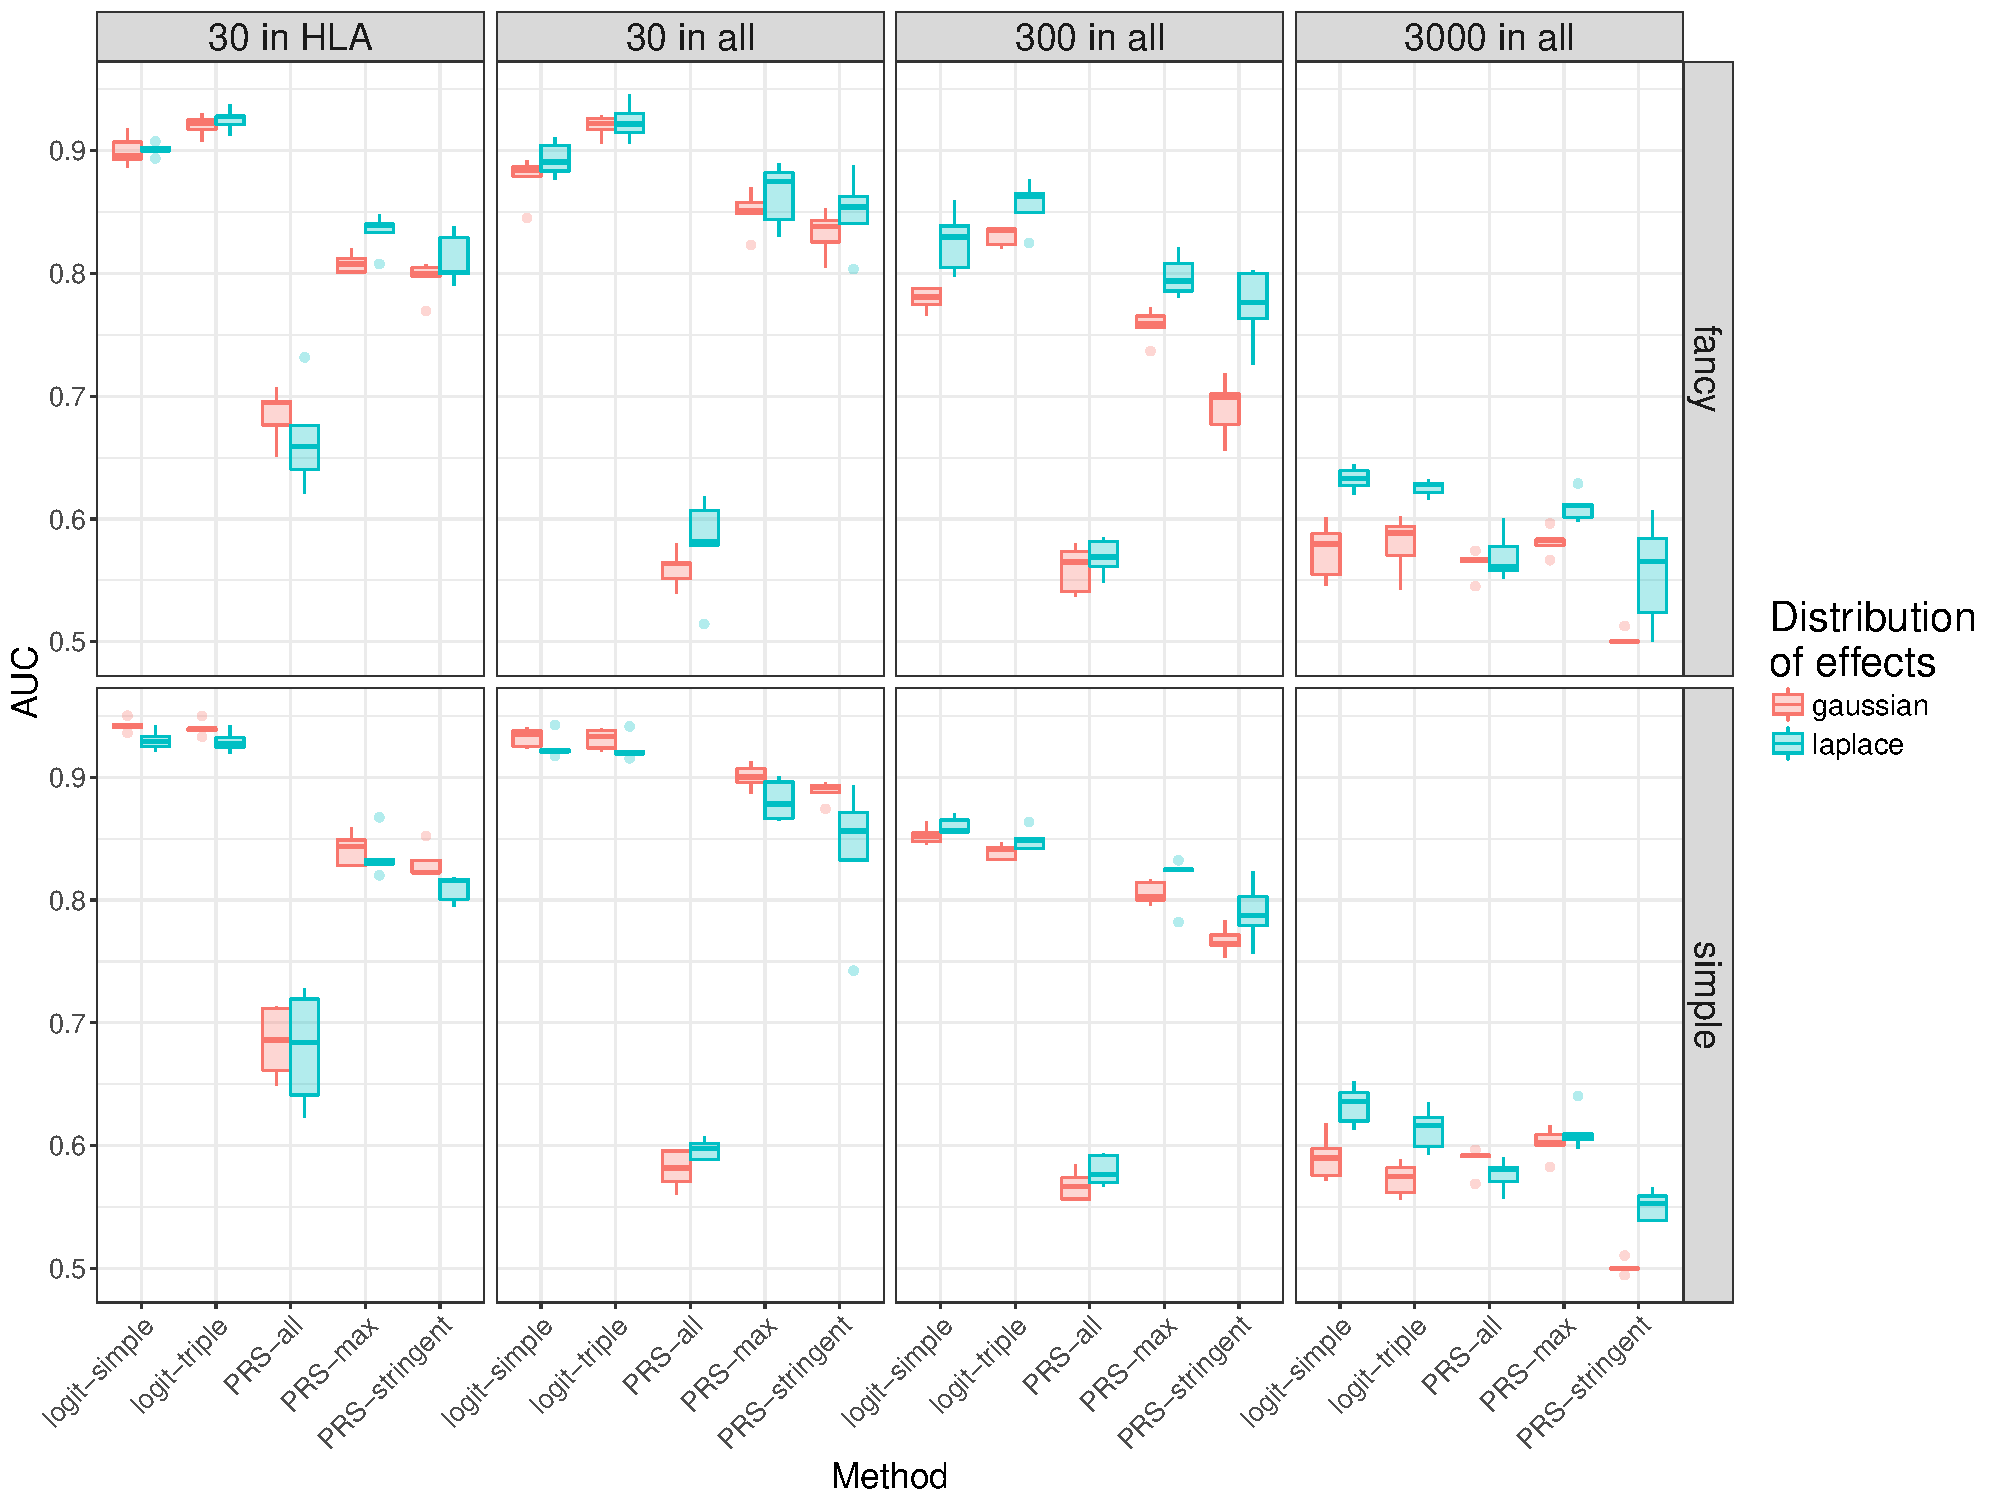
\includegraphics[width=\textwidth]{AUC}}
\caption{AUC...}\label{fig:AUC}
\end{figure}

\newpage
\begin{figure}[h]
\centerline{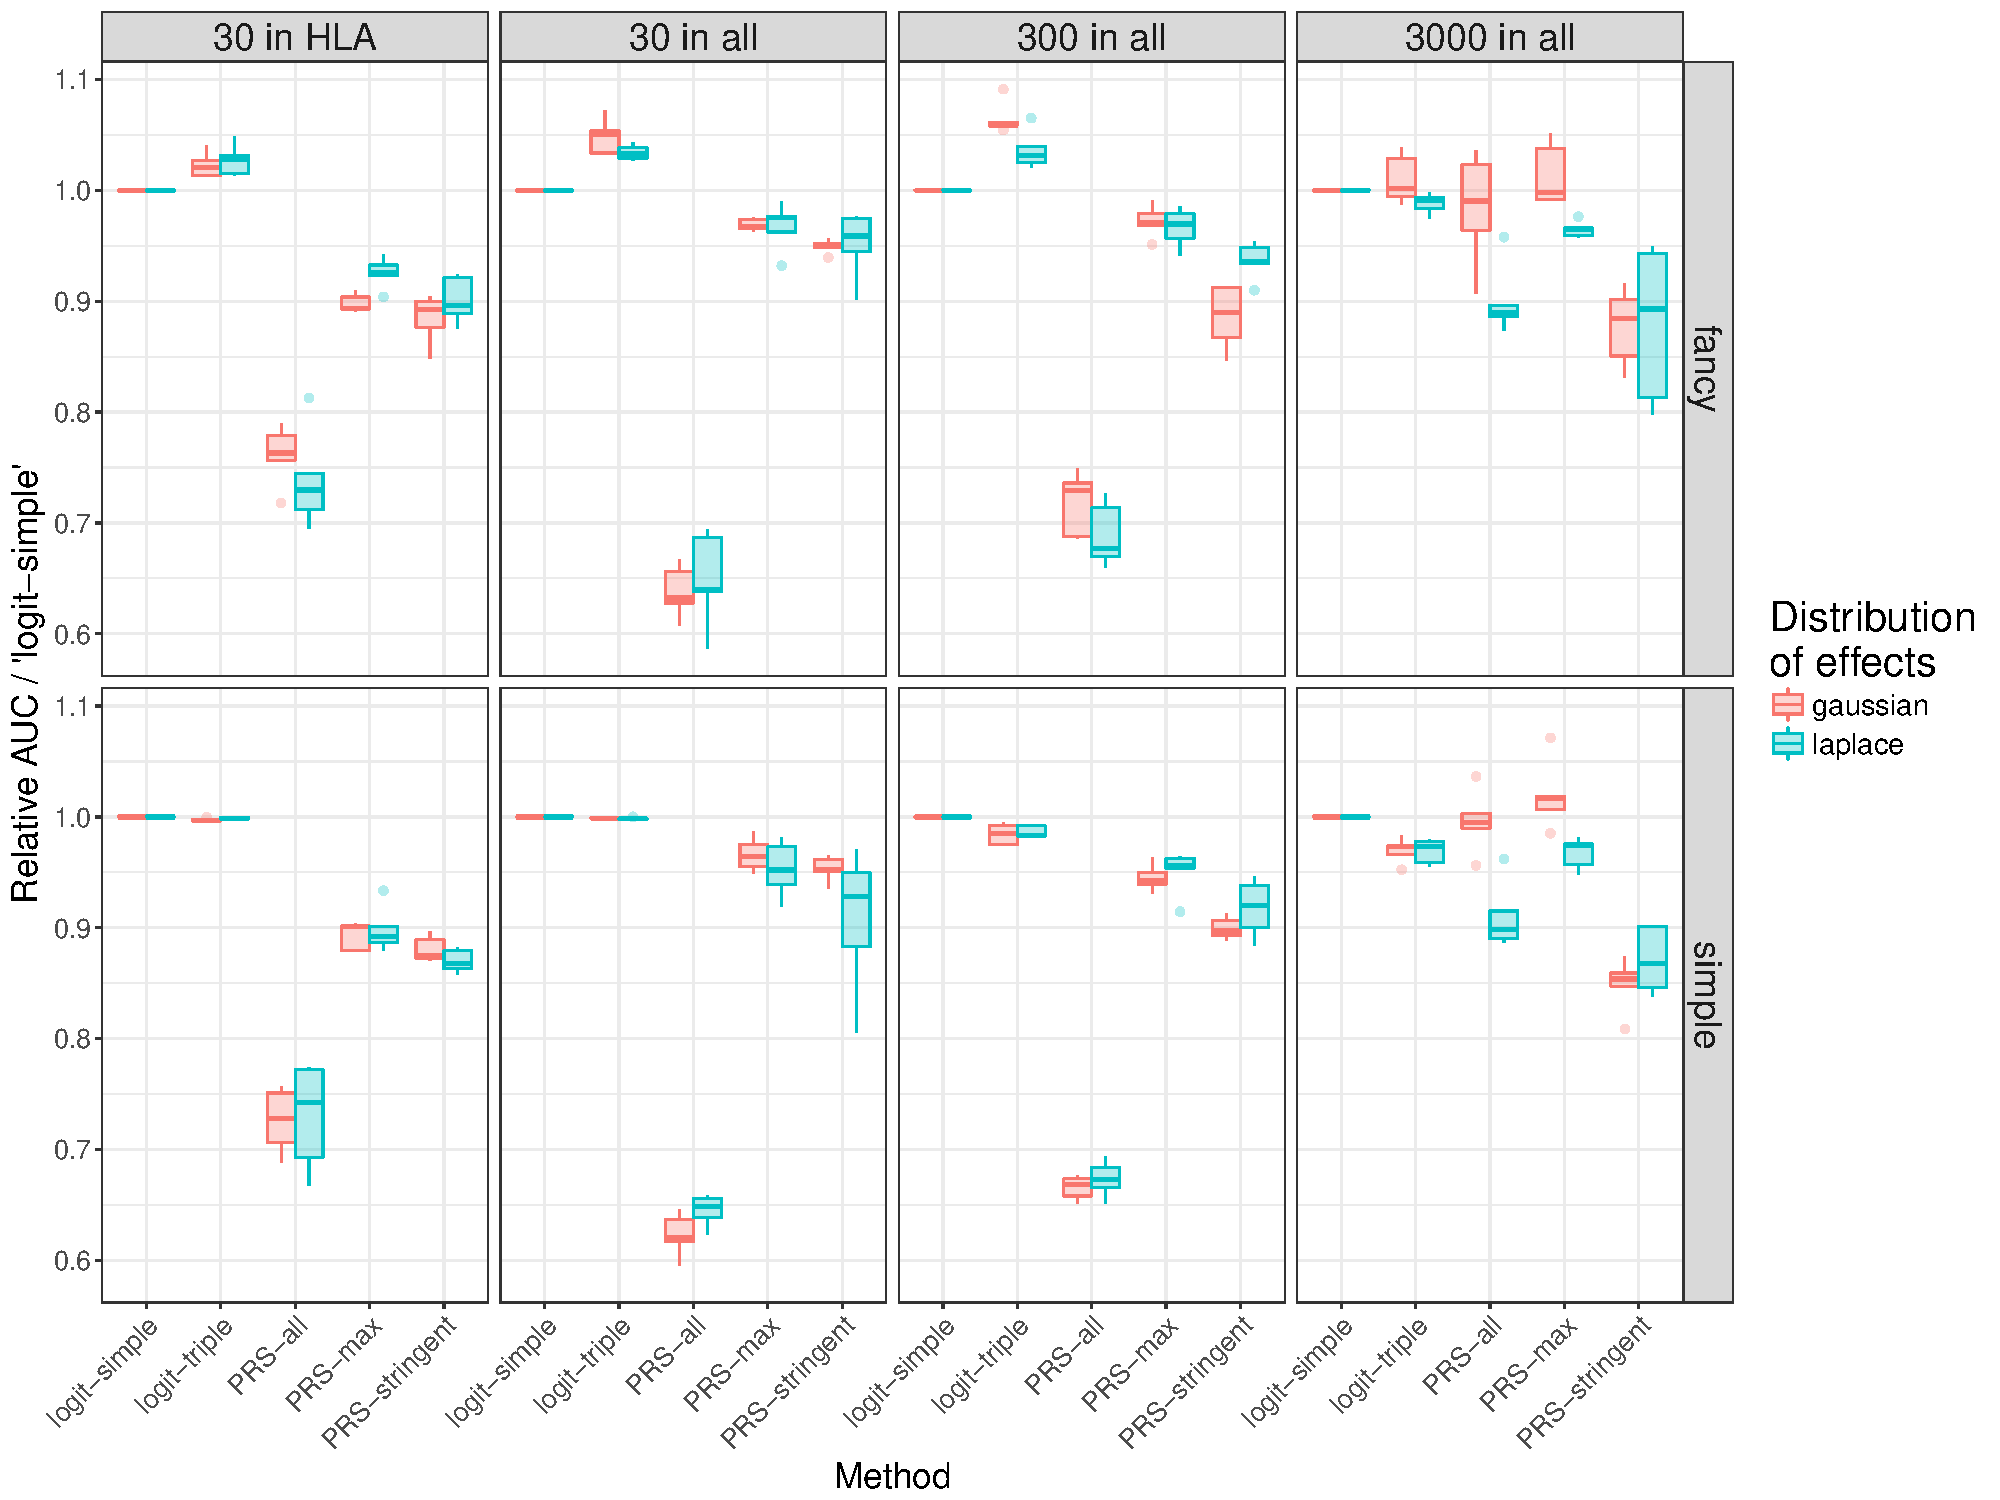
\includegraphics[width=\textwidth]{AUC-rel}}
\caption{Relative AUC...}\label{fig:AUC-rel}
\end{figure}

%%%%%%%%%%%%%%%%%%%%%%%%%%%%%%%%%%%%%%%%%%%%%%%%%%%%%%%%%%%%%%%%%%%%%%%%%%%%%%%%

\newpage
\section*{Acknowledgements}

Authors acknowledge Grenoble Alpes Data Institute, supported by the French National Research Agency under the ``Investissements d'avenir'' program (ANR-15-IDEX-02) and the LabEx PERSYVAL-Lab (ANR-11-LABX-0025-01). We are also grateful to F\'elix Balazard for useful discussions about T-Trees.

\vspace*{-12pt}

\bibliographystyle{natbib}
\bibliography{refs}

%%%%%%%%%%%%%%%%%%%%%%%%%%%%%%%%%%%%%%%%%%%%%%%%%%%%%%%%%%%%%%%%%%%%%%%%%%%%%%%%

\newpage
\section*{Supplementary Data}

\renewcommand{\thefigure}{S\arabic{figure}}
\setcounter{figure}{0}
\renewcommand{\thetable}{S\arabic{table}}
\setcounter{table}{0}

%%%%%%%%%%%%%%%%%%%%%%%%%%%%%%%%%%%%%%%%%%%%%%%%%%%%%%%%%%%%%%%%%%%%%%%%%%%%%%%%

\begin{table}[ht]
\centering
\begin{tabular}{|l|cccc|r|}
\hline
Population & UK & Finland & Netherlands & Italy & Total\\
\hline
Cases & 2569 & 637 & 795 & 495 & 4496\\
Controls & 7492 & 1799 & 828 & 540 & 10659\\
\hline
Total & 10061 & 2436 & 1623 & 1035 & 15155\\
\hline
\end{tabular}
\caption{Number of individuals by population and disease status for the celiac disease cohort (after quality control, genotyped on 281,122 ..mutual.. SNPs).}
\label{tab:celiac-data}
\end{table}

%%%%%%%%%%%%%%%%%%%%%%%%%%%%%%%%%%%%%%%%%%%%%%%%%%%%%%%%%%%%%%%%%%%%%%%%%%%%%%%%

% latex table generated in R 3.4.1 by xtable 1.8-2 package
% Thu Oct 26 16:46:26 2017
\begin{table}[ht]
\centering
\begin{tabular}{ccccccccccccccc}
  \hline
1.00e+00 & 7.22e-01 & 5.87e-01 & 4.20e-01 & 2.43e-01 & 1.00e-01 & 2.35e-02 & 2.21e-03 & 4.69e-05 & 8.81e-08 & 3.18e-12 & 1.83e-19 & 2.89e-31 & 1.70e-50 & 7.71e-82 \\ 
  5.00e-08 & 7.05e-01 & 5.65e-01 & 3.95e-01 & 2.20e-01 & 8.47e-02 & 1.79e-02 & 1.42e-03 & 2.28e-05 & 2.73e-08 & 4.69e-13 & 8.08e-21 & 1.80e-33 & 4.30e-54 & 1.06e-87 \\ 
  7.94e-01 & 6.87e-01 & 5.42e-01 & 3.69e-01 & 1.97e-01 & 7.08e-02 & 1.34e-02 & 8.83e-04 & 1.05e-05 & 7.74e-09 & 6.03e-14 & 2.86e-22 & 7.73e-36 & 5.97e-58 & 5.49e-94 \\ 
  7.81e-01 & 6.69e-01 & 5.19e-01 & 3.43e-01 & 1.75e-01 & 5.85e-02 & 9.79e-03 & 5.31e-04 & 4.61e-06 & 2.01e-09 & 6.69e-15 & 7.92e-24 & 2.24e-38 & 4.37e-62 & 1.00e-100 \\ 
  7.67e-01 & 6.50e-01 & 4.95e-01 & 3.18e-01 & 1.54e-01 & 4.76e-02 & 7.01e-03 & 3.08e-04 & 1.90e-06 & 4.72e-10 & 6.32e-16 & 1.70e-25 & 4.26e-41 & 1.61e-66 &  \\ 
  7.53e-01 & 6.30e-01 & 4.70e-01 & 2.93e-01 & 1.35e-01 & 3.82e-02 & 4.90e-03 & 1.72e-04 & 7.31e-07 & 1.00e-10 & 5.04e-17 & 2.75e-27 & 5.16e-44 & 2.83e-71 &  \\ 
  7.38e-01 & 6.09e-01 & 4.46e-01 & 2.68e-01 & 1.17e-01 & 3.02e-02 & 3.33e-03 & 9.18e-05 & 2.63e-07 & 1.89e-11 & 3.35e-18 & 3.31e-29 & 3.84e-47 & 2.26e-76 &  \\ 
   \hline
\end{tabular}
\caption{The 102 thresholds used in the P+T method for this study.}
\label{tab:thr}
\end{table}

%%%%%%%%%%%%%%%%%%%%%%%%%%%%%%%%%%%%%%%%%%%%%%%%%%%%%%%%%%%%%%%%%%%%%%%%%%%%%%%%

\begin{figure}[h]
\centerline{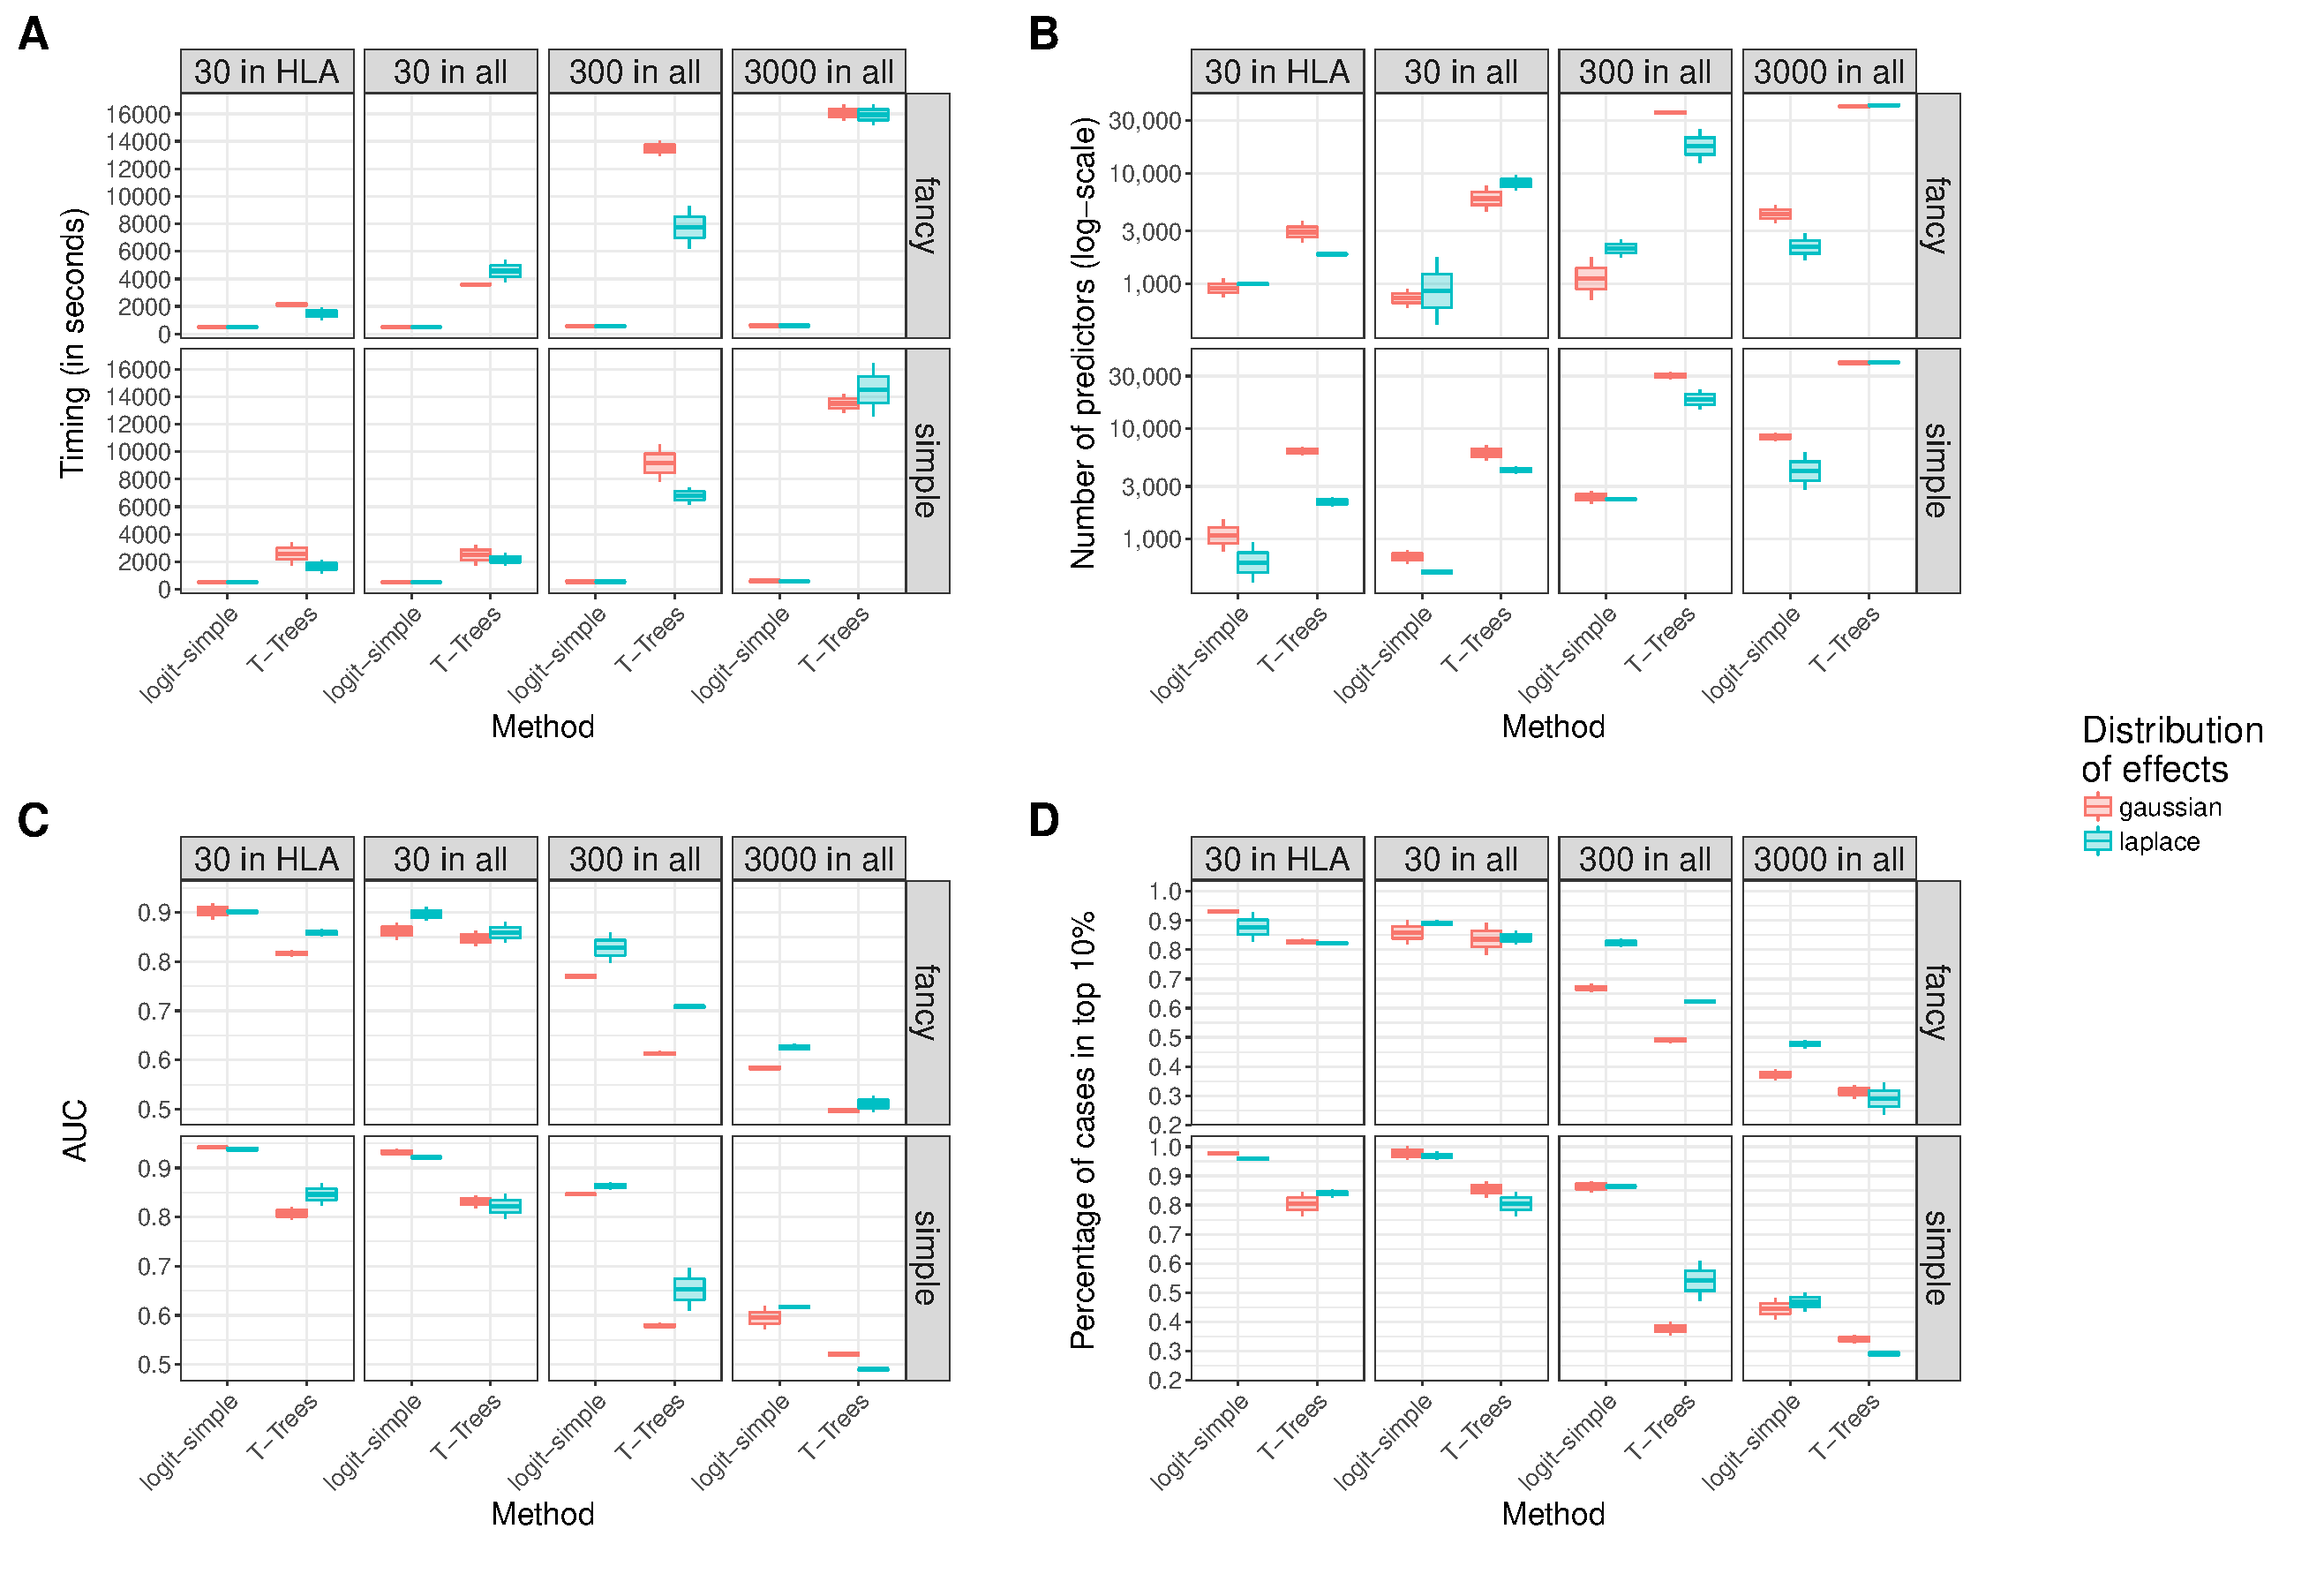
\includegraphics[width=\textwidth]{ttrees}}
\caption{Results of T-Trees vs penalized logistic regression. \textbf{A.} Timing (in seconds). \textbf{B.} Number of predictors of the model. \textbf{C.} AUC. \textbf{D.} Percentage of cases in the 10\% largest scores.}\label{fig:ttrees}
\end{figure}

%%%%%%%%%%%%%%%%%%%%%%%%%%%%%%%%%%%%%%%%%%%%%%%%%%%%%%%%%%%%%%%%%%%%%%%%%%%%%%%%

\begin{figure}[h]
\centerline{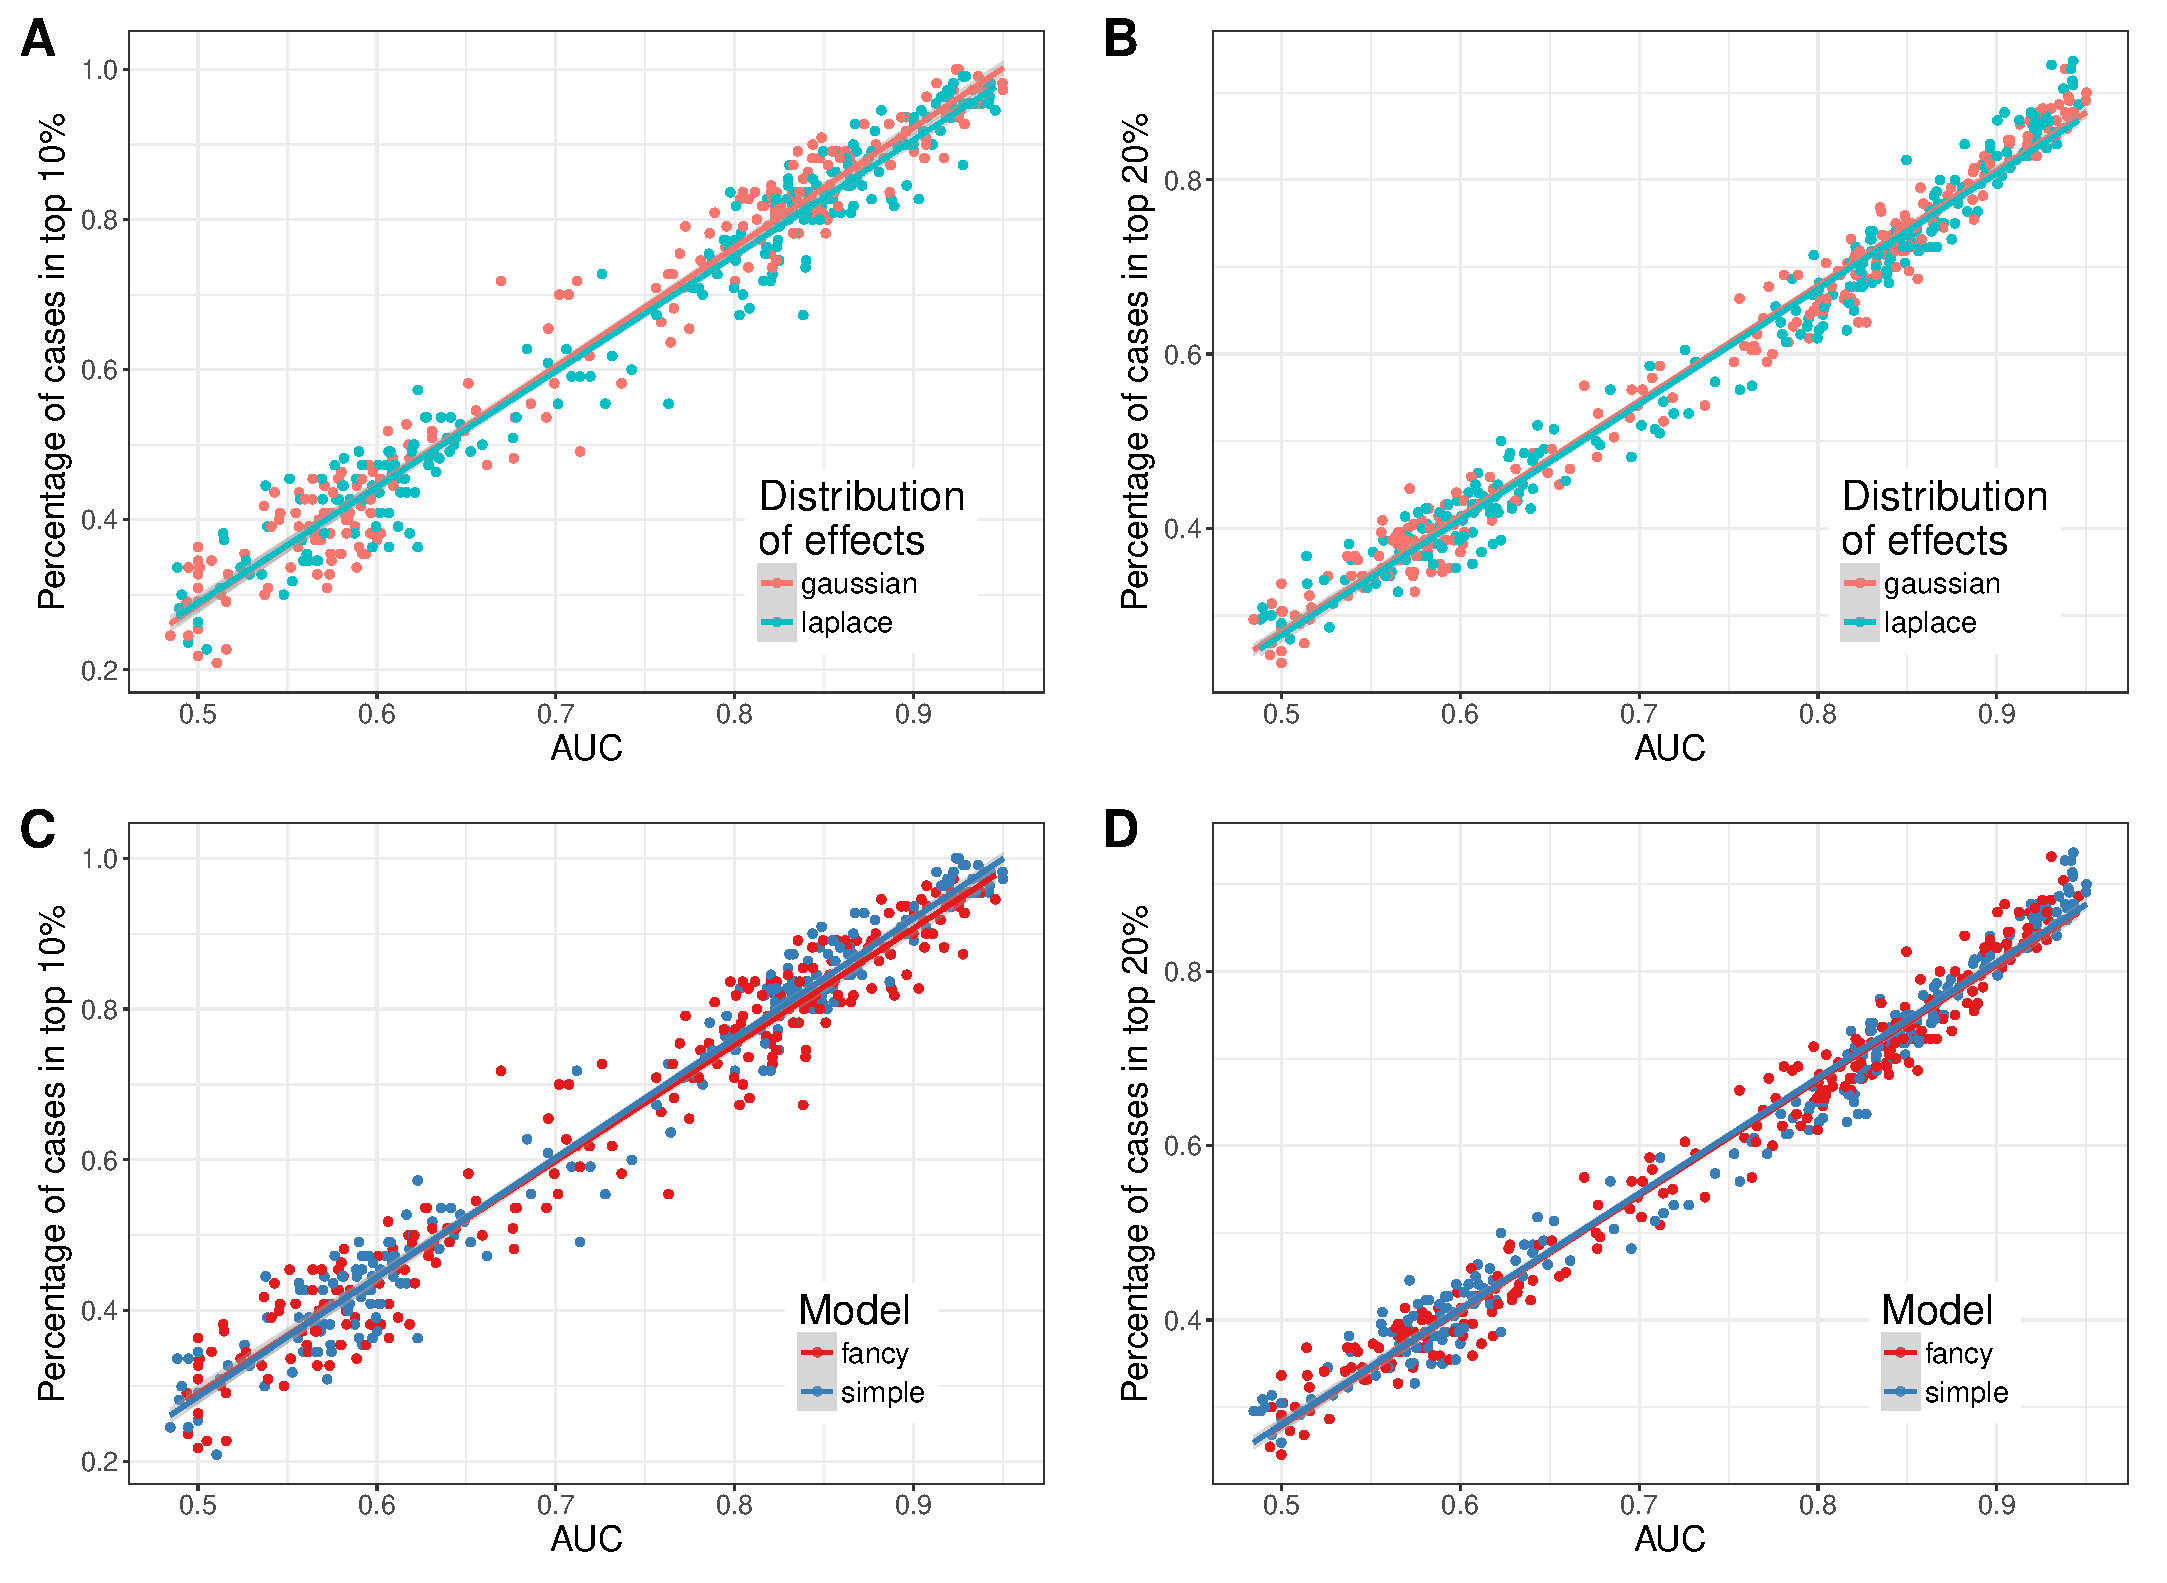
\includegraphics[width=\textwidth]{AUC-corr}}
\caption{Percentage of cases in the 2 highest deciles of PRSs as a function of AUC.}\label{fig:AUC-corr}
\end{figure}

%%%%%%%%%%%%%%%%%%%%%%%%%%%%%%%%%%%%%%%%%%%%%%%%%%%%%%%%%%%%%%%%%%%%%%%%%%%%%%%%

\begin{figure}[h]
\centerline{
\includegraphics[width=\textwidth]{meme}}
\caption{Meme to use on Twitter when promoting the preprint?}\label{fig:meme}
\end{figure}

\end{document}
